\documentclass[10pt,twocolumn,letterpaper]{article}

\usepackage[T1]{fontenc}
\usepackage{mathptmx}
\usepackage[letterpaper,margin=0.75in,columnsep=0.25in]{geometry}
\usepackage{amsmath,amssymb,amsthm,mathtools,bm}
\usepackage{graphicx}
\usepackage{booktabs}
\usepackage[font=small,labelfont=bf]{caption}
\usepackage{microtype}
\usepackage{xcolor}
\usepackage{enumitem}
\usepackage{algorithm}
\usepackage{algpseudocode}
\usepackage[round,authoryear]{natbib}
\usepackage[colorlinks=true,linkcolor=blue!50!black,citecolor=blue!50!black,urlcolor=blue!50!black]{hyperref}
\usepackage[capitalise,noabbrev]{cleveref}

% ---- Submission settings ------------------------------------------------------
\newif\ifanonymous
\anonymousfalse   % \anonymoustrue for double-blind review: hides authors and the code link
\newcommand{\paperauthors}{Author names}  % TODO: authors and affiliations
\newcommand{\coderepo}{\url{https://github.com/maomlab/capfid}}
% -------------------------------------------------------------------------------

\setlist{nosep,leftmargin=*}
\raggedbottom
\newtheorem{proposition}{Proposition}
\newtheorem{corollary}{Corollary}
\theoremstyle{definition}
\newtheorem{definition}{Definition}
\theoremstyle{remark}
\newtheorem{remark}{Remark}

\newcommand{\KL}{\mathrm{KL}}
\newcommand{\tr}{\operatorname{tr}}
\newcommand{\logdet}{\log\det}
\newcommand{\Vol}{\mathcal{V}}
\newcommand{\Inf}{\mathcal{I}}
\newcommand{\N}{\mathcal{N}}
\newcommand{\D}{\mathcal{D}}
\newcommand{\DS}{\mathcal{D}_{\setminus S}}
\newcommand{\Di}{\mathcal{D}_{\setminus i}}
\newcommand{\T}{^{\top}}
\newcommand{\dof}{d}

\title{\vspace{-1.2em}\Large\bf How Many Bits Does a Training Example Cost?\\
Per-Example Capacity versus Fidelity via Linearized Laplace Unlearning}
\author{\ifanonymous Anonymous Author(s)\\ {\small Submission under review; do not distribute}\else\paperauthors\fi}
\date{}

\begin{document}
\maketitle

\begin{abstract}
The compression/fidelity trade-off is usually stated for a whole model: parameters are a code whose length is traded against the code length of the data given those parameters. We ask the per-example version of the question: how much of a trained network's capacity is spent on each training example (or set of examples), and how well is that example fit? We define capacity by \emph{unlearning}: the change in a linearized Laplace posterior over the weights when an example is removed, measured as (i) the effective number of parameters it determines, (ii) the drop in posterior differential entropy (a label-agnostic \emph{volume}), and (iii) the Kullback--Leibler divergence between the posteriors with and without it (the label-dependent \emph{information} actually stored). All three reduce to $C\times C$ output-space matrices, so every example is scored after a single factorization, and arbitrary sets are scored jointly. Under exact Bayesian updating, information capacity equals the example's generalization gap (training minus held-out log-likelihood); volume equals the mutual information between weights and label for Gaussian likelihoods; and volume is submodular, which yields a redundancy ratio for sets. In a closed-form linear model all identities hold to $10^{-13}$ bits. On a two-moons MLP with 10\% flipped labels, sweeping the prior precision moves flipped examples from \emph{ignored} (low fidelity, $\sim$0.08 bits each) to \emph{memorized} (high fidelity, $\sim$1.6 bits each), while the Laplace evidence favors the most compressed model. On a 4{,}130-parameter vision transformer trained on $8\times 8$ digits with 5\% flipped labels, flipped examples cost a median of 3.5 bits versus 0.05 bits for clean ones, 14 of the 16 most expensive images are flips, and capacity rank-correlates with memorization measured by actual retraining (Spearman 0.84--0.88). The one-step held-out prediction, however, overestimates the effect of removing heavily memorized examples by up to several-fold, which we document as the main limitation.\ifanonymous\else{} Code: \coderepo.\fi
\end{abstract}

\section{Introduction}
Minimum description length (MDL) and the information bottleneck frame learning as a trade-off between how much information a model stores and how faithfully it reproduces data \citep{rissanen1978,hinton1993,tishby2000,grunwald2007}. A model with a short parameter code that explains the data well generalizes; a model that stores many bits to fit a few examples memorizes. These statements are global. In practice one often wants the \emph{per-example} decomposition: which examples consume capacity, how much, and what the model gets in return in fidelity. This matters for auditing memorization \citep{zhang2017,feldman2020,feldman2020neural}, diagnosing label noise, identifying long-tail subpopulations, and valuing data \citep{ghorbani2019,pruthi2020,covert2024}, a question economists study as the value of information \citep{raiffa1961,abadie2023}.

Two families of tools approximate pieces of this picture. Influence functions estimate how parameters or predictions change when an example is removed \citep{cook1977,koh2017}, and memorization scores compare held-in and held-out likelihood, typically by retraining many models \citep{feldman2020neural}. Information-theoretic work defines the information an example leaves in the weights through the divergence between weight distributions trained with and without it \citep{achille2019,harutyunyan2021}. We build on the last line and make three things explicit: a family of capacity measures with distinct meanings, identities that tie them to fidelity and to classical quantities, and a two-dimensional \emph{capacity--fidelity} diagnostic that can be computed for every example of a small network in seconds.

\paragraph{Contributions.}
\begin{itemize}
\item We define three nested per-example (and per-set) capacity measures by Laplace unlearning: effective degrees of freedom, volume (entropy drop), and information (KL), and show they reduce exactly to $C\times C$ output-space quantities (\cref{prop:reduction}).
\item We prove or collect identities that give them meaning: information equals the generalization gap under exact Bayesian updating (\cref{prop:bayes}); volume equals the weight--label mutual information for Gaussian likelihoods and the leverage formula $-\tfrac12\log(1-h_{ii})$ in linear regression; per-example degrees of freedom sum to MacKay's effective number of parameters; and volume is submodular, giving a redundancy ratio $\ge 1$ for sets and an upper bound on the fraction of model information attributable to single examples (\cref{prop:submod}).
\item We connect the totals to a Laplace two-part MDL code (\cref{sec:mdl}) and demonstrate the diagnostic on an exactly solvable model, an MLP under a prior-precision sweep, and a small vision transformer, validating against warm-started retraining and documenting where the approximation fails.
\end{itemize}

\section{Background and related work}
\paragraph{Laplace approximations.} The Laplace approximation fits a Gaussian at a mode using the curvature of the negative log posterior \citep{mackay1992}. For neural networks the generalized Gauss--Newton (GGN) curvature is positive semidefinite and corresponds to a linearization of the network in its parameters \citep{ritter2018,immer2021,daxberger2021}. The Laplace marginal likelihood penalizes models by an Occam factor that MacKay related to the effective number of well-determined parameters, $\gamma$.

\paragraph{Leverage and influence.} In linear regression the diagonal $h_{ii}$ of the hat matrix measures how much an observation determines its own fit, and $\sum_i h_{ii}$ is the model's degrees of freedom \citep{hoaglin1978,cook1977}. Influence functions generalize the parameter shift to differentiable models \citep{koh2017}, but are known to be fragile for deep networks, especially for highly influential points \citep{basu2021,bae2022}.

\paragraph{Information in the weights and generalization.} \citet{achille2019} define the information a dataset stores in the weights as a KL to a prior, and \citet{harutyunyan2021} introduced \emph{smooth unique information}: a KL between weight distributions trained with and without an example, computed with a linearized network. Information-theoretic generalization bounds control the gap between train and test loss by the mutual information between weights and individual examples \citep{xu2017,bu2020}. Our \cref{prop:bayes} is the pointwise, exact-posterior version of this connection. MDL views of deep learning \citep{hinton1993,blier2018} motivate reading the Laplace evidence as a two-part code.

\paragraph{Value of information and the economics of data.} Statistical decision theory values data by what it does for decisions: the expected value of sample information is the expected improvement in the payoff of the best action after observing data, net of the cost of collecting it \citep{blackwell1951,raiffa1961,howard1966}. \citet{abadie2023} turned this into an empirical-Bayes estimator of the value of evidence-based decision making. A decision maker with prior $\tau\sim\N(\mu,\gamma^2)$ on a policy's payoff can buy a signal $\hat\tau\sim\N(\tau,\sigma^2)$ and launch only if the posterior mean is positive; the value of evidence is the resulting gain in expected payoff minus its cost, estimated from many past experiments. They show how this value changes with statistical precision and that launch rules based on statistical significance can leave it unrealized. Two connections to our measures are exact. First, when the utility is the logarithmic score of a reported belief about the parameters, the expected value of an experiment is its expected KL divergence from prior to posterior, that is, the mutual information between parameters and data \citep{lindley1956,bernardo1979}. By \cref{cor:mi}, our volume $\Vol(S)$ is exactly this quantity for the labels of $S$ given the rest of the data (for Gaussian likelihoods): it is the \emph{ex ante} value of those labels to such a decision maker, and $\Inf(S)$ is their \emph{ex post} value once observed. Second, in their Gaussian model the value of evidence depends on precision only through the shrinkage weight $h=\gamma^2/(\gamma^2+\sigma^2)$, which is the single-observation leverage $K$ of \cref{prop:reduction}; the corresponding volume is $-\tfrac12\log(1-h)=\tfrac12\log(1+\gamma^2/\sigma^2)$. The frameworks differ in what is valued. Theirs prices evidence by a downstream decision and its cost; ours prices training examples in model capacity and fit, with no decision layer. Selecting $\alpha$ by maximizing the Laplace evidence (\cref{sec:mdl}), which we report but did not use to set $\alpha$, would be the same empirical-Bayes step they use to estimate the prior from a population of studies.

\paragraph{Data valuation, scaling laws, and large language models.} Data valuation in machine learning assigns each example a share of held-out performance, for example through Shapley values \citep{ghorbani2019} or gradient tracing \citep{pruthi2020}. \citet{covert2024} found that an example's marginal contribution to performance shrinks log-linearly with the size of the dataset it joins, with example-specific exponents: some examples matter most in small datasets and others remain useful in large ones. Our capacity is an information-theoretic counterpart of their marginal contribution, evaluated at the full dataset (a subset of size $N-1$) and measured as information stored rather than held-out loss. With curvatures held at $\theta^*$, \cref{prop:submod} implies that an example's marginal volume can only shrink as the dataset it joins grows, the diminishing returns their scaling laws quantify, and the Laplace approximation gives this marginal volume in closed form for any subset, so information-scaling curves could be traced without retraining. At the largest scale, influence functions with eigenvalue-corrected Kronecker-factored curvature have been applied to language models with up to 52 billion parameters to trace behaviors back to pretraining documents \citep{grosse2023}. The same curvature approximations are the natural route to scaling our capacity measures (\cref{sec:compute}).

\section{Method}
\subsection{Setup}
Let $\D=\{(x_i,y_i)\}_{i=1}^N$, $f(x;\theta)\in\mathbb{R}^C$ a network with $\theta\in\mathbb{R}^P$, and $\ell(y,f)=-\log p(y\mid f)$. We train a MAP estimate $\theta^*$ of
\begin{equation}
L(\theta)=\textstyle\sum_{i=1}^N \ell\big(y_i,f(x_i;\theta)\big)+\tfrac{\alpha}{2}\|\theta\|^2,
\label{eq:objective}
\end{equation}
i.e., a summed loss with a Gaussian prior $\N(0,\alpha^{-1}I)$. At $\theta^*$ define the Jacobian $J_i=\partial f(x_i)/\partial\theta\in\mathbb{R}^{C\times P}$, the output-space residual $r_i=\nabla_f\ell\in\mathbb{R}^C$, and curvature $\Lambda_i=\nabla^2_f\ell\in\mathbb{R}^{C\times C}$ (for softmax, $r_i=p_i-e_{y_i}$ and $\Lambda_i=\mathrm{diag}(p_i)-p_ip_i\T$). The linearized Laplace posterior is
\begin{equation}
q_\D=\N(\theta^*,\Sigma),\qquad \Sigma^{-1}=A=\textstyle\sum_i J_i\T\Lambda_iJ_i+\alpha I.
\label{eq:laplace}
\end{equation}

\paragraph{Unlearning a set.} For $S\subseteq[N]$ with $m=|S|$, stack $J_S\in\mathbb{R}^{mC\times P}$, $r_S\in\mathbb{R}^{mC}$, and $\Lambda_S=\mathrm{blkdiag}(\Lambda_i)_{i\in S}$. Removing $S$ subtracts its curvature and, because $\nabla L(\theta^*)=0$, one Newton step on $L-\sum_{i\in S}\ell_i$ gives
\begin{equation}
A_{-S}=A-J_S\T\Lambda_SJ_S,\qquad \theta^*_{-S}=\theta^*+A_{-S}^{-1}J_S\T r_S,
\label{eq:unlearn}
\end{equation}
and $q_{\DS}=\N(\theta^*_{-S},A_{-S}^{-1})$. This is exact for linear-Gaussian models.

\subsection{Capacity and fidelity}
\begin{definition}[Capacity]\label{def:capacity}
For a set $S$,
\begin{align*}
\dof(S)&=\tr\!\big(\Sigma\,J_S\T\Lambda_SJ_S\big) &&\text{(degrees of freedom)}\\
\Vol(S)&=h(q_{\DS})-h(q_\D) &&\text{(volume)}\\
\Inf(S)&=\KL\big(q_\D\,\|\,q_{\DS}\big) &&\text{(information)}
\end{align*}
with $h$ the differential entropy. We report $\Vol$ and $\Inf$ in bits.
\end{definition}
$\Vol$ is the log-ratio of weight-space volumes the examples pin down; it depends on the inputs and on the rest of the data, but not on the labels $y_S$ except through $\Lambda_S$. $\Inf$ adds a mean-shift term and measures what is actually stored about the labeled examples. Unlike an absolute differential entropy, $\Vol$ is invariant to affine reparameterizations of $\theta$ (and, within the Laplace approximation, to any smooth reparameterization, which is linearized at $\theta^*$ so that the Jacobian terms cancel); $\Inf$ is invariant to any bijection.

\begin{definition}[Fidelity]
The fidelity of example $i$ is $F_i=\log_2 p(y_i\mid x_i,\theta^*)$ and its held-out fidelity is $F_i^{-}=\log_2 p(y_i\mid x_i,\theta^*_{-i})$, using the linearized held-out logits of \cref{prop:reduction}. Posterior-averaged versions are $\bar F_i=\mathbb{E}_{q_\D}\log_2 p(y_i\mid\theta)$ and $\tilde F^{-}_i=\log_2\mathbb{E}_{q_{\Di}}p(y_i\mid\theta)$.
\end{definition}

\begin{proposition}[Output-space reduction]\label{prop:reduction}
Let $S_S=J_S\Sigma J_S\T$, $K_S=\Lambda_S^{1/2}S_S\Lambda_S^{1/2}$ and $S_{-S}=J_SA_{-S}^{-1}J_S\T=S_S+S_S\Lambda_S^{1/2}(I-K_S)^{-1}\Lambda_S^{1/2}S_S$. Then, in nats,
\begin{align*}
\dof(S)&=\tr K_S,\qquad \Vol(S)=-\tfrac12\logdet(I-K_S),\\
\Inf(S)&=\tfrac12\Big[r_S\T S_{-S}\,r_S-\tr K_S-\logdet(I-K_S)\Big],
\end{align*}
and the linearized held-out logits are $f(x_S)+S_{-S}r_S$.
\end{proposition}
All quantities involve only $mC\times mC$ matrices; for single examples they are $C\times C$. The proof (\cref{app:proofs}) uses Sylvester's determinant identity and the Woodbury identity. $K_S$ is a block of the posterior ``hat'' matrix: it is the leverage of $S$ under the Laplace posterior. Since $A_{-S}\succeq\alpha I$, the eigenvalues of $K_S$ lie in $[0,1)$.

\begin{proposition}[Information is the generalization gap]\label{prop:bayes}
If $q_\D\propto q_{\DS}\,p(y_S\mid\theta)$ exactly, then
\[
\Inf(S)=\mathbb{E}_{q_\D}\big[\log p(y_S\mid\theta)\big]-\log\mathbb{E}_{q_{\DS}}\big[p(y_S\mid\theta)\big].
\]
\end{proposition}
That is, the bits the posterior stores about $S$ equal the difference between its posterior-averaged training fit and its leave-$S$-out predictive fit. The condition holds for linear-Gaussian models, where \cref{eq:unlearn} is exact. On a plot of $\bar F_i$ against $\Inf(\{i\})$, lines of slope one are then iso-lines of held-out likelihood.

\begin{corollary}[Volume as mutual information]\label{cor:mi}
For a Gaussian likelihood, $\Sigma$ does not depend on $y$, and $\mathbb{E}_{y_S\sim p(\cdot\mid \DS)}\Inf(S)=\Vol(S)=I(\theta;y_S\mid x_S,\DS)$. For linear regression with a Gaussian prior, $\Vol(\{i\})=-\tfrac12\log(1-h_{ii})$ where $h_{ii}$ is the leverage of the Bayesian ridge hat matrix.
\end{corollary}
So $\Vol$ is the \emph{capacity allotted} to an input location (the expected information about any plausible label), while $\Inf$ is the information spent on the observed label. Expanding in the eigenvalues $\kappa$ of $K_S$: $\Vol\approx\tfrac12\sum\kappa$, whereas the covariance part of $\Inf$ is $\tfrac12\sum[-\kappa-\log(1-\kappa)]\approx\tfrac14\sum\kappa^2$. For well-fit examples (small $r$), $\Inf\approx\Vol^2$ in nats: they occupy volume but store little. Examples with surprising labels add the mean-shift term and can have $\Inf>\Vol$.

\paragraph{Degrees of freedom.} Summed over single examples, $\sum_i\dof(\{i\})=\tr(\Sigma\,\mathrm{GGN})=P-\alpha\tr\Sigma=\gamma$, MacKay's effective number of parameters. Thus $\dof(\{i\})$ is example $i$'s share of the model's capacity in parameter units.

\begin{proposition}[Redundancy]\label{prop:submod}
For every $S$, $\Vol(S)\ge\sum_{i\in S}\Vol(\{i\})$, and the total model information $\Vol_{\mathrm{tot}}=h(\text{prior})-h(q_\D)=\tfrac12\logdet(I+\mathrm{GGN}/\alpha)$ satisfies $\sum_{i=1}^N\Vol(\{i\})\le\Vol_{\mathrm{tot}}$.
\end{proposition}
This follows from submodularity of $T\mapsto\logdet(\alpha I+\sum_{i\in T}J_i\T\Lambda_iJ_i)$ \citep{krause2008}. We report the \emph{redundancy ratio} $\rho(S)=\Vol(S)/\sum_{i\in S}\Vol(\{i\})\ge1$, which is large when members of $S$ encode the same information, and the \emph{unique fraction} $u=\sum_i\Vol(\{i\})/\Vol_{\mathrm{tot}}\le1$.

\subsection{Totals as a two-part code}\label{sec:mdl}
The Laplace log evidence decomposes as $-\log p(\D)\approx L_{\text{data}}+L_{\text{model}}$ with $L_{\text{data}}=-\sum_i\log p(y_i\mid x_i,\theta^*)$ and $L_{\text{model}}=\tfrac{\alpha}{2}\|\theta^*\|^2+\Vol_{\mathrm{tot}}$. Moreover $\KL(q_\D\|\text{prior})=L_{\text{model}}-\gamma/2$. Varying $\alpha$ moves along a compression/fidelity curve, and the evidence selects a point on it.

\subsection{Computation}\label{sec:compute}
\begin{algorithm}[t]
\caption{Per-example capacity and fidelity}\label{alg:main}
\begin{algorithmic}[1]
\State $J\gets$ per-example Jacobians ($N\times C\times P$; \texttt{vmap(jacrev)})
\State $A\gets\alpha I+\sum_i J_i\T\Lambda_iJ_i$;\; $L\gets\mathrm{chol}(A)$
\For{each batch $B$}
  \State $V\gets L^{-1}J_B\T$;\; $S_i\gets V_i\T V_i$ for $i\in B$
\EndFor
\For{each $i$ (batched $C\times C$ algebra)}
  \State $K_i,\ S_{-i},\ \dof,\ \Vol,\ \Inf$ via \cref{prop:reduction}
  \State $F_i$ from $f(x_i)$;\; $F_i^{-}$ from $f(x_i)+S_{-i}r_i$
\EndFor
\end{algorithmic}
\end{algorithm}
\Cref{alg:main} costs $O(NCP^2+P^3)$ time and $O(P^2+NCP)$ memory for the exact GGN; set capacities need one extra triangular solve with $J_S\T$. Expectations over $q$ use Monte Carlo with common random numbers. The method is implemented in the open-source PyTorch package \texttt{capfid} (see Code availability). For larger models, only $J_i\Sigma J_i\T$ is needed, so Kronecker-factored, last-layer, or low-rank curvature can be substituted \citep{martens2015,ritter2018,daxberger2021}.

\section{Experiments}
All experiments ran on a single CPU core in double-precision Laplace algebra; details are in \cref{app:details}.

\subsection{Exact check: Bayesian linear regression}
We fit $N=200$ noisy samples of $\sin(2x)$ with $P=40$ random Fourier features ($\sigma=0.3$, $\alpha=1$; five targets shifted by $+2$ as outliers) and compared \cref{prop:reduction,prop:bayes} and \cref{cor:mi} with brute-force refits without each point (\cref{tab:exact}). All agree to numerical precision. Per-example degrees of freedom sum to $\tr H=9.091$ effective parameters, and outliers carry a mean of 1.34 bits versus 0.044 bits for inliers.

\begin{table}[t]
\centering\small
\caption{Exact check in Bayesian linear regression: maximum absolute discrepancy over all 200 examples.}\label{tab:exact}
\begin{tabular}{@{}lr@{}}
\toprule
Quantity & max error (bits)\\
\midrule
$\Inf$ (\cref{prop:reduction}) vs.\ exact refit KL & $1.6\times10^{-13}$\\
held-out log-lik vs.\ exact refit & $2.8\times10^{-14}$\\
$\Inf$ vs.\ train $-$ held-out (\cref{prop:bayes}) & $9.6\times10^{-15}$\\
$\Vol$ vs.\ $-\frac12\log_2(1-h_{ii})$ (\cref{cor:mi}) & $3.9\times10^{-16}$\\
\midrule
$\sum_i\dof(\{i\})$ vs.\ $\tr H$ & 9.091 vs.\ 9.091\\
\bottomrule
\end{tabular}
\end{table}

\begin{figure*}[t]
\centering
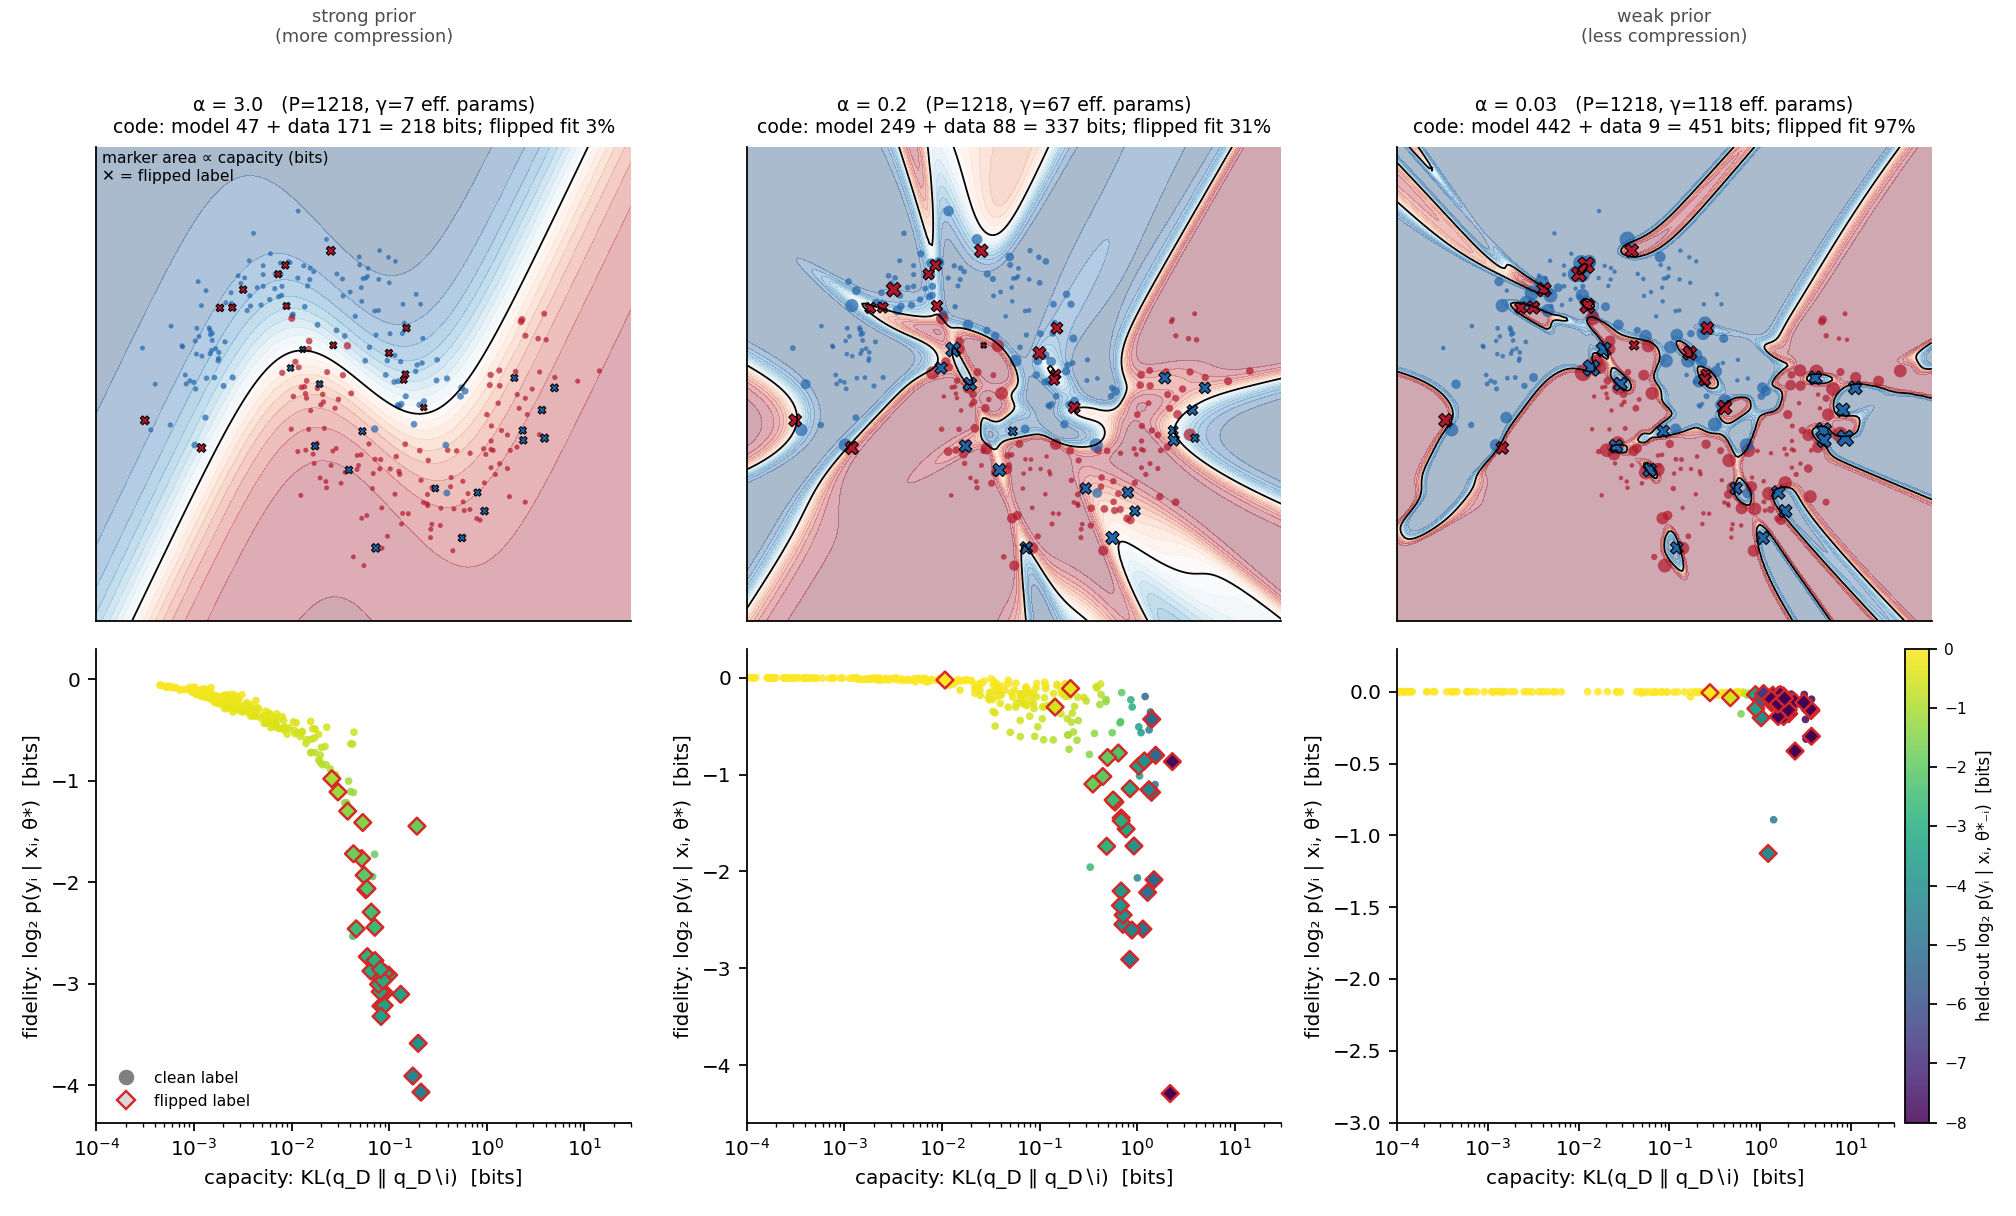
\includegraphics[width=0.94\textwidth]{figures/fig1_moons_capacity_vs_fidelity.png}
\caption{\textbf{Two moons with 32/300 flipped labels, tanh MLP ($P=1218$), sweeping the prior precision $\alpha$.} Top: decision function; marker area $\propto\Inf(\{i\})$; $\times$ marks flipped labels. Bottom: capacity $\Inf(\{i\})$ versus fidelity $F_i$; color is the predicted held-out fidelity $F_i^{-}$; diamonds with red edges are flipped labels. Titles give the two-part code $L_{\text{model}}+L_{\text{data}}$ in bits. As the prior weakens, flipped examples move from \emph{ignored} (low fidelity, held-out $\approx$ fidelity) to \emph{memorized} (high fidelity, $\sim$1--4 bits each, low held-out fidelity) and carve islands in the decision boundary.}
\label{fig:moons}
\end{figure*}

\subsection{Compression sweep: two moons}
We trained a 2--32--32--2 tanh MLP ($P=1218$) on 300 two-moons points with 32 flipped labels at $\alpha\in\{3,0.2,0.03\}$ (\cref{fig:moons}, \cref{tab:moons}). Weakening the prior increases the effective parameters from 6.8 to 118.5 and moves flipped examples from ignored (1/32 fit) to memorized (31/32 fit). The median capacity of a flipped example rises from 0.078 to 1.59 bits, while clean examples stay between 0.001 and 0.02 bits. Total code length grows from 218 to 451 bits: the decrease in data bits (171$\to$9) is outweighed by the increase in model bits (47$\to$442), so the Laplace evidence prefers the most compressed model, the one that ignores the noise. Only 31--51\% of the total model information is attributable to single examples.

\begin{table}[t]
\centering\small
\setlength{\tabcolsep}{2.6pt}
\caption{Two-moons prior-precision sweep. $L$ values in bits; $\tilde\Inf$ is the median of $\Inf(\{i\})$ (bits); $u$ is the unique fraction (\cref{prop:submod}).}\label{tab:moons}
\begin{tabular}{@{}lrrrrrcrrr@{}}
\toprule
$\alpha$ & $\gamma$ & $\Vol_{\mathrm{tot}}$ & $L_{\text{model}}$ & $L_{\text{data}}$ & total & flips fit & $\tilde\Inf_{\text{flip}}$ & $\tilde\Inf_{\text{clean}}$ & $u$\\
\midrule
3    & 6.8   & 16  & 47  & 171 & 218 & 1/32  & 0.078 & 0.0024 & 0.31\\
0.2  & 66.6  & 201 & 249 & 88  & 337 & 10/32 & 0.744 & 0.0199 & 0.32\\
0.03 & 118.5 & 414 & 442 & 9   & 451 & 31/32 & 1.585 & 0.0013 & 0.51\\
\bottomrule
\end{tabular}
\end{table}

A side observation: at $\alpha=0.03$ the posterior-averaged fidelity $\bar F_i$ reached $-41$ bits for some examples that $\theta^*$ fits well. For confident examples $\Lambda_i\to0$, so the Gaussian's tails extend into regions of very low likelihood. We therefore plot the plug-in fidelity $F_i$; the capacity measures are unaffected.

\subsection{A small vision transformer on digits}
We trained a one-block vision transformer (2$\times$2 patches, 16 tokens plus a class token, width 20, two heads; $P=4130$) on 1{,}000 of scikit-learn's $8\times8$ digits \citep{pedregosa2011} with 63 labels flipped to a random other class, at $\alpha=8$ (\cref{fig:vit}). The model reached 0.875 test accuracy and fit 58/63 flipped labels, with $\gamma=847$ effective parameters. Flipped examples cost a median of 3.46 bits versus 0.049 bits for clean ones (71$\times$). Of the 16 highest-capacity images, 14 are flips; the other two are atypical but correctly labeled digits (a ``2'' and an ``8''), which is the long-tail behavior predicted by \citet{feldman2020}. Clean examples follow the $\Inf\approx\Vol^2$ regime (slope two in \cref{fig:vit}b), while flips lie above it. The unique fraction is $u=0.38$.

Removing a whole digit class costs 14--25\% more volume than the sum of its members' single-example volumes ($\rho=1.14$--$1.25$), whereas the flipped set ($\rho=1.07$) and a random clean set of the same size ($\rho=1.02$) are nearly additive (\cref{tab:sets}). Members of a class redundantly encode shared structure; flipped labels and random examples do not. The joint $\Inf$ shows the same ordering more strongly (class ratios 1.8--3.3 versus 1.1 for flips), but it relies on a large joint Newton step and is less reliable than $\Vol$, which depends only on curvature.

\begin{figure*}[t]
\centering
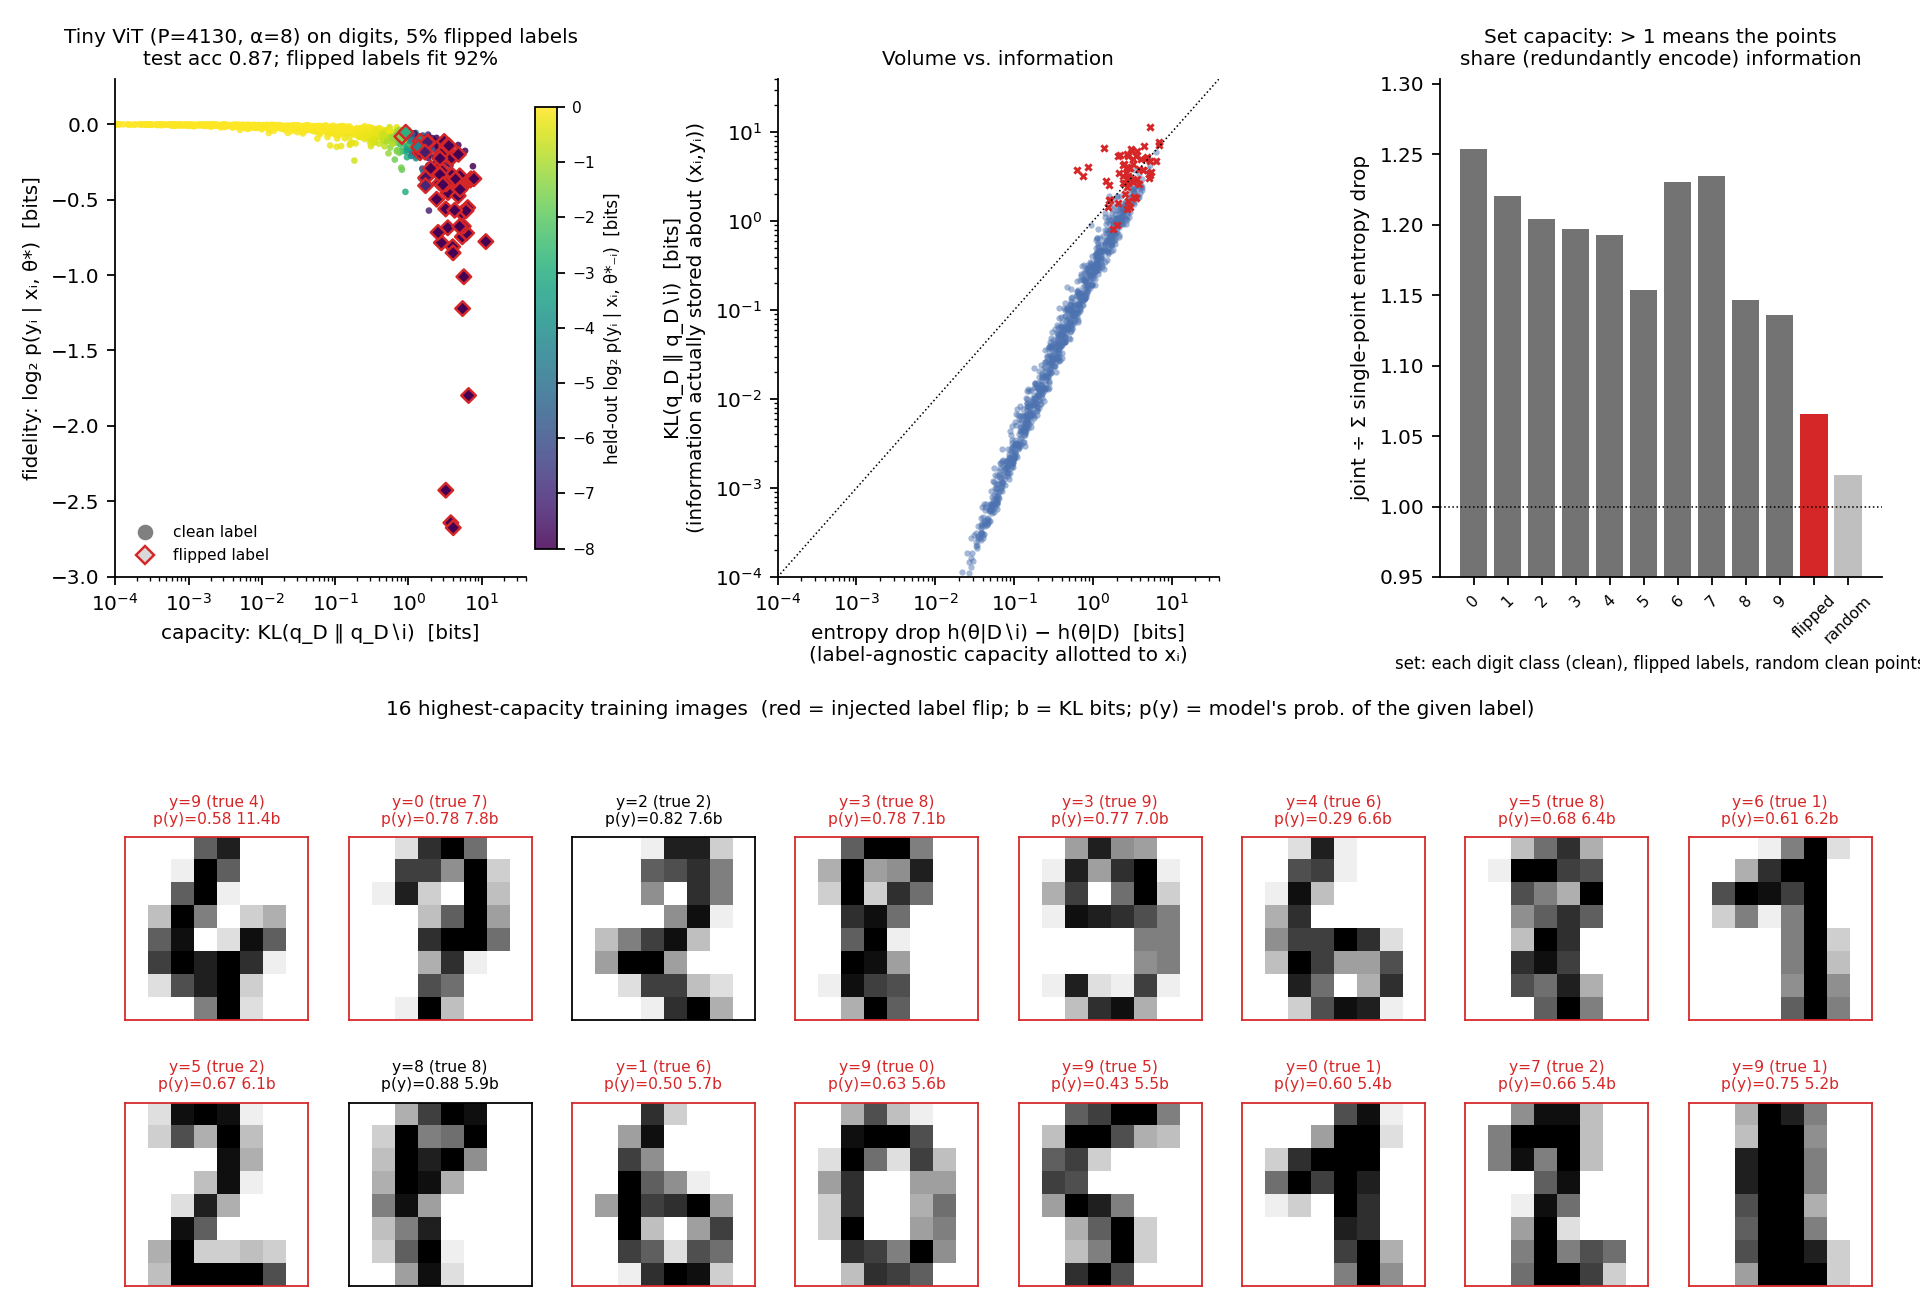
\includegraphics[width=0.94\textwidth]{figures/fig2_vit_digits.png}
\caption{\textbf{Vision transformer ($P=4130$, $\alpha=8$) on $8\times8$ digits with 63/1000 flipped labels.} (a) Capacity versus fidelity, colored by predicted held-out fidelity. (b) Volume $\Vol$ versus information $\Inf$ per example: clean examples (blue) follow $\Inf\approx\Vol^2$ (in nats); flips (red) store more than their volume. (c) Redundancy ratio $\rho(S)$ for each clean digit class, the flipped set, and a random clean set of equal size. (d) The 16 highest-capacity training images with given and true labels, the model's probability of the given label, and $\Inf$ in bits; red frames are injected flips.}
\label{fig:vit}
\end{figure*}

\begin{table}[t]
\centering\small
\setlength{\tabcolsep}{3.5pt}
\caption{Set capacities (bits) for the transformer. ``joint'' removes the set at once; ``sum'' adds single-example values. $\rho$ is the volume redundancy ratio.}\label{tab:sets}
\begin{tabular}{@{}lrrrrrr@{}}
\toprule
set & $n$ & $\Vol$ joint & $\Vol$ sum & $\rho$ & $\Inf$ joint & $\Inf$ sum\\
\midrule
class 0 & 94  & 71.4  & 56.9  & 1.25 & 62.7  & 19.2\\
class 1 & 95  & 119.4 & 97.8  & 1.22 & 116.6 & 46.0\\
class 2 & 81  & 78.2  & 65.0  & 1.20 & 69.7  & 30.3\\
class 3 & 102 & 113.1 & 94.5  & 1.20 & 93.0  & 42.5\\
class 4 & 91  & 68.0  & 57.0  & 1.19 & 57.9  & 22.9\\
class 5 & 101 & 72.2  & 62.6  & 1.15 & 53.2  & 27.1\\
class 6 & 83  & 88.0  & 71.5  & 1.23 & 66.4  & 28.4\\
class 7 & 102 & 82.9  & 67.1  & 1.24 & 74.4  & 28.7\\
class 8 & 95  & 102.3 & 89.2  & 1.15 & 81.7  & 41.5\\
class 9 & 93  & 84.5  & 74.4  & 1.14 & 57.2  & 32.4\\
\midrule
flipped & 63  & 213.4 & 200.2 & 1.07 & 267.9 & 242.1\\
random  & 63  & 44.1  & 43.1  & 1.02 & 17.2  & 15.9\\
\bottomrule
\end{tabular}
\end{table}

\subsection{Validation against retraining}
For 40 MLP examples ($\alpha=0.2$; the 20 highest-capacity and 20 random) and 28 transformer examples (12 highest and 16 random), we retrained without each example by warm-started L-BFGS and measured actual memorization $F_i-\log_2p(y_i\mid x_i,\theta^{\text{retrain}}_{-i})$ (\cref{fig:val}). Capacity ranks actual memorization well: Spearman correlation between $\Inf(\{i\})$ and actual memorization is 0.84 (MLP) and 0.88 (transformer), monotone over four orders of magnitude. The one-step prediction of memorization, $F_i-F_i^{-}$, is accurate for typical examples but not for heavily memorized ones. For all 12 highest-capacity transformer examples it overestimated (about 17--60 predicted versus 6--13 actual bits), and for the MLP it was scattered on both sides of the diagonal (Pearson 0.60 overall, 0.90 for the transformer, the latter driven largely by the separation between groups). This matches reports that influence approximations degrade for highly influential points \citep{basu2021,bae2022}. Computing all 1{,}000 transformer capacities took about 11\,s, less than one warm-started retrain ($\approx$14\,s).

\begin{figure*}[t]
\centering
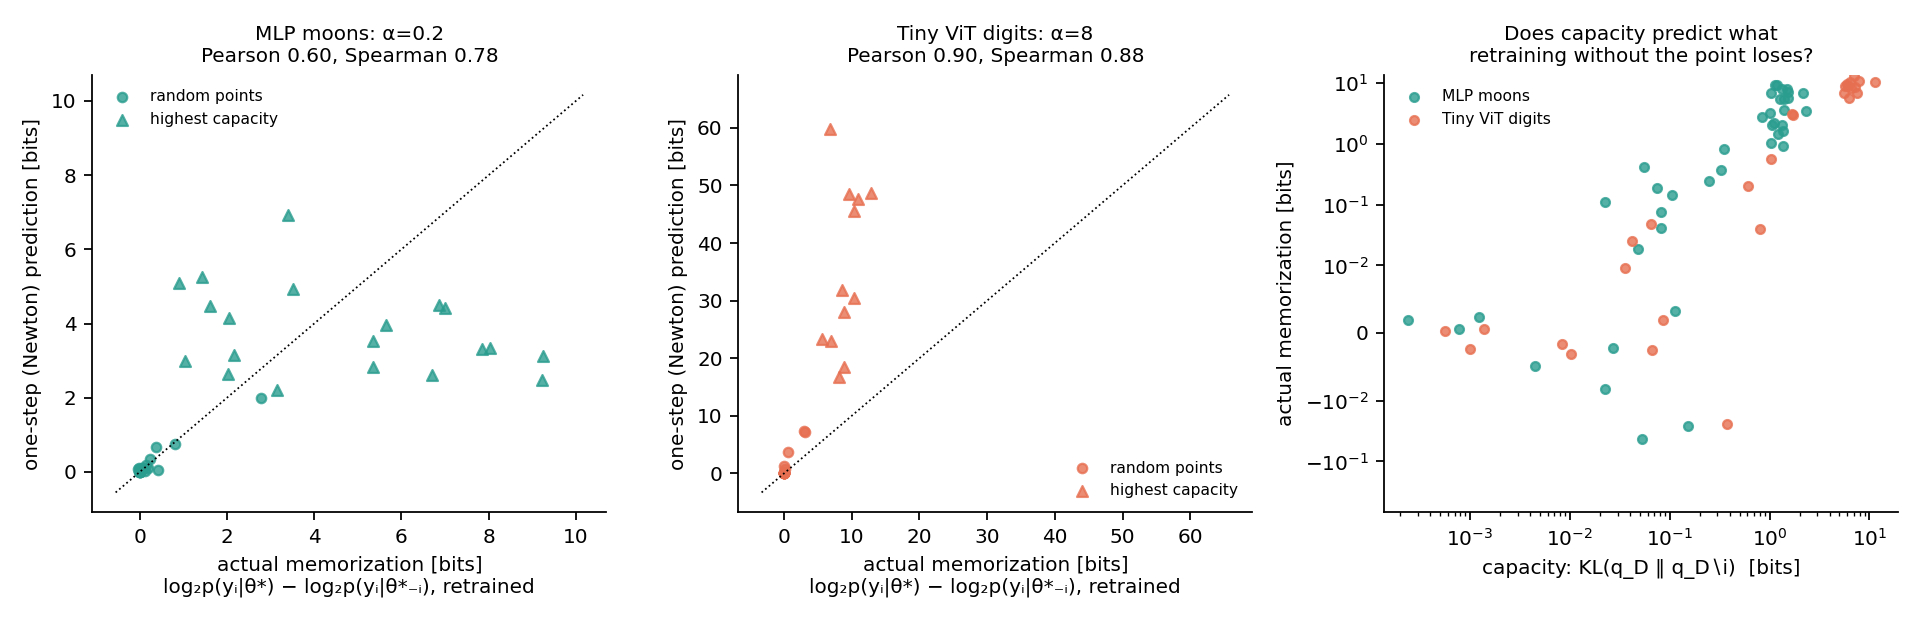
\includegraphics[width=0.94\textwidth]{figures/fig3_validation.png}
\caption{\textbf{Validation against warm-started retraining.} Left, middle: one-step (Newton) prediction of memorization versus actual memorization for the MLP ($\alpha=0.2$) and the transformer ($\alpha=8$); triangles are the highest-capacity examples. Right: capacity $\Inf(\{i\})$ versus actual memorization for both models (symmetric-log $y$ axis).}
\label{fig:val}
\end{figure*}

\section{Discussion and limitations}
\paragraph{A taxonomy.} The capacity--fidelity plane separates (i) \emph{typical} examples (low capacity, high fidelity, held-out $\approx$ fidelity), (ii) \emph{memorized} examples (high capacity, high fidelity, low held-out fidelity), (iii) \emph{ignored} examples (modest capacity, low fidelity), and (iv) \emph{atypical but correct} examples (elevated capacity, high fidelity), the long tail that memorization may legitimately serve \citep{feldman2020}. The prior precision moves examples between (iii) and (ii), and the evidence offers a principled stopping point.

\paragraph{Limitations.}
\begin{itemize}
\item \emph{Locality.} The Laplace posterior describes one basin and ignores the implicit regularization of stochastic training; capacities are defined relative to a prior, as any MDL code requires a precision.
\item \emph{One-step unlearning.} Held-out predictions for heavily memorized examples are miscalibrated (up to several-fold); treat capacity as a ranking and held-out fidelity as qualitative in that regime. Joint KL for large sets inherits this problem.
\item \emph{Over-dispersion.} Posterior-averaged likelihoods are pessimistic for confident networks at weak priors; this does not affect $\Vol$, $\Inf$, or $\dof$.
\item \emph{Scale and scope.} Exact GGN limits us to $P\lesssim10^4$; results use single seeds, small models, and priors chosen by hand (\cref{app:details}). Kronecker-factored curvature has made influence functions tractable for language models with tens of billions of parameters \citep{grosse2023}, but whether capacity estimates remain reliable at that scale is untested.
\end{itemize}

\paragraph{Unique versus shared information.} Leave-one-out quantities measure only \emph{unique} information; \cref{prop:submod} shows they undercount the total, by about half to two-thirds here. A Shapley-style average over removal orders would distribute $\Vol_{\mathrm{tot}}$ exactly and is a natural extension. Tracing each example's marginal volume across nested subsets of increasing size would give an information-theoretic counterpart of individualized data scaling laws \citep{covert2024}. It would also test a hypothesis our class-level results suggest but do not establish: that examples in redundant groups (high $\rho$) are those whose value decays fastest with dataset size, while flipped and atypical examples retain unique information as the dataset grows.

\section{Conclusion}
Defining per-example capacity by Laplace unlearning yields three interpretable quantities (degrees of freedom, volume, and information) that are exact in linear-Gaussian models, cheap to compute for every example, tied to the generalization gap and to the MDL code length, and empirically predictive of which examples a network has memorized. Plotted against fidelity, they give a direct, per-example view of where a model spends its capacity.

Capacity is the cost side of a per-example ledger. Value-of-information analyses in economics \citep{abadie2023} and data-valuation and scaling analyses in machine learning \citep{ghorbani2019,covert2024} measure the benefit side: the improvement in downstream decisions or held-out performance that an example buys. The two coincide under a logarithmic utility, where volume is the expected value of an example's label, but not in general. In our experiments, memorizing flipped labels consumed capacity and lengthened the total description of the data, a machine-learning analogue of evidence with negative net value. Measuring costs and benefits on a common scale in bits, and tracking how both scale with dataset size, is a natural next step.

\section*{Code availability}
\ifanonymous
The implementation, unit tests, and scripts that regenerate every figure and table are provided as anonymized supplementary material and will be released publicly upon publication.
\else
The method is implemented in \texttt{capfid}, an MIT-licensed PyTorch package available at \coderepo. The repository includes unit tests that check \cref{prop:reduction,prop:bayes,prop:submod} and \cref{cor:mi} against brute-force refits, and the script \texttt{examples/paper/reproduce\_paper.py}, which regenerates every figure and table in this paper.
\fi

\begingroup
\small
\setlength{\bibsep}{2pt}
\begin{thebibliography}{40}

\bibitem[Abadie et~al.(2023)]{abadie2023}
A.~Abadie, A.~Agarwal, G.~Imbens, S.~Jia, J.~McQueen, S.~Stepaniants, and S.~Torres.
\newblock Estimating the value of evidence-based decision making.
\newblock \emph{arXiv:2306.13681}, 2023.

\bibitem[Achille et~al.(2019)Achille, Paolini, and Soatto]{achille2019}
A.~Achille, G.~Paolini, and S.~Soatto.
\newblock Where is the information in a deep neural network?
\newblock \emph{arXiv:1905.12213}, 2019.

\bibitem[Bae et~al.(2022)]{bae2022}
J.~Bae, N.~Ng, A.~Lo, M.~Ghassemi, and R.~Grosse.
\newblock If influence functions are the answer, then what is the question?
\newblock In \emph{NeurIPS}, 2022.

\bibitem[Basu et~al.(2021)Basu, Pope, and Feizi]{basu2021}
S.~Basu, P.~Pope, and S.~Feizi.
\newblock Influence functions in deep learning are fragile.
\newblock In \emph{ICLR}, 2021.

\bibitem[Bernardo(1979)]{bernardo1979}
J.~M. Bernardo.
\newblock Expected information as expected utility.
\newblock \emph{The Annals of Statistics}, 7(3):686--690, 1979.

\bibitem[Blackwell(1951)]{blackwell1951}
D.~Blackwell.
\newblock Comparison of experiments.
\newblock In \emph{Proceedings of the Second Berkeley Symposium on Mathematical Statistics and Probability}, pages 93--102, 1951.

\bibitem[Blier and Ollivier(2018)]{blier2018}
L.~Blier and Y.~Ollivier.
\newblock The description length of deep learning models.
\newblock In \emph{NeurIPS}, 2018.

\bibitem[Bu et~al.(2020)Bu, Zou, and Veeravalli]{bu2020}
Y.~Bu, S.~Zou, and V.~V. Veeravalli.
\newblock Tightening mutual information-based bounds on generalization error.
\newblock \emph{IEEE Journal on Selected Areas in Information Theory}, 1(1):121--130, 2020.

\bibitem[Cook(1977)]{cook1977}
R.~D. Cook.
\newblock Detection of influential observation in linear regression.
\newblock \emph{Technometrics}, 19(1):15--18, 1977.

\bibitem[Covert et~al.(2024)Covert, Ji, Hashimoto, and Zou]{covert2024}
I.~Covert, W.~Ji, T.~Hashimoto, and J.~Zou.
\newblock Scaling laws for the value of individual data points in machine learning.
\newblock In \emph{ICML}, PMLR 235:9380--9406, 2024.

\bibitem[Daxberger et~al.(2021)]{daxberger2021}
E.~Daxberger, A.~Kristiadi, A.~Immer, R.~Eschenhagen, M.~Bauer, and P.~Hennig.
\newblock Laplace redux: Effortless {B}ayesian deep learning.
\newblock In \emph{NeurIPS}, 2021.

\bibitem[Feldman(2020)]{feldman2020}
V.~Feldman.
\newblock Does learning require memorization? {A} short tale about a long tail.
\newblock In \emph{STOC}, 2020.

\bibitem[Feldman and Zhang(2020)]{feldman2020neural}
V.~Feldman and C.~Zhang.
\newblock What neural networks memorize and why: Discovering the long tail via influence estimation.
\newblock In \emph{NeurIPS}, 2020.

\bibitem[Ghorbani and Zou(2019)]{ghorbani2019}
A.~Ghorbani and J.~Zou.
\newblock Data {S}hapley: Equitable valuation of data for machine learning.
\newblock In \emph{ICML}, 2019.

\bibitem[Grosse et~al.(2023)]{grosse2023}
R.~Grosse, J.~Bae, C.~Anil, N.~Elhage, A.~Tamkin, A.~Tajdini, B.~Steiner, D.~Li, E.~Durmus, E.~Perez, E.~Hubinger, K.~Luko{\v{s}}i{\=u}t{\.e}, K.~Nguyen, N.~Joseph, S.~McCandlish, J.~Kaplan, and S.~R. Bowman.
\newblock Studying large language model generalization with influence functions.
\newblock \emph{arXiv:2308.03296}, 2023.

\bibitem[Gr{\"u}nwald(2007)]{grunwald2007}
P.~D. Gr{\"u}nwald.
\newblock \emph{The Minimum Description Length Principle}.
\newblock MIT Press, 2007.

\bibitem[Harutyunyan et~al.(2021)]{harutyunyan2021}
H.~Harutyunyan, A.~Achille, G.~Paolini, O.~Majumder, A.~Ravichandran, R.~Bhotika, and S.~Soatto.
\newblock Estimating informativeness of samples with smooth unique information.
\newblock In \emph{ICLR}, 2021.

\bibitem[Hinton and van Camp(1993)]{hinton1993}
G.~E. Hinton and D.~van Camp.
\newblock Keeping the neural networks simple by minimizing the description length of the weights.
\newblock In \emph{COLT}, 1993.

\bibitem[Hoaglin and Welsch(1978)]{hoaglin1978}
D.~C. Hoaglin and R.~E. Welsch.
\newblock The hat matrix in regression and {ANOVA}.
\newblock \emph{The American Statistician}, 32(1):17--22, 1978.

\bibitem[Howard(1966)]{howard1966}
R.~A. Howard.
\newblock Information value theory.
\newblock \emph{IEEE Transactions on Systems Science and Cybernetics}, 2(1):22--26, 1966.

\bibitem[Immer et~al.(2021)Immer, Korzepa, and Bauer]{immer2021}
A.~Immer, M.~Korzepa, and M.~Bauer.
\newblock Improving predictions of {B}ayesian neural nets via local linearization.
\newblock In \emph{AISTATS}, 2021.

\bibitem[Koh and Liang(2017)]{koh2017}
P.~W. Koh and P.~Liang.
\newblock Understanding black-box predictions via influence functions.
\newblock In \emph{ICML}, 2017.

\bibitem[Krause et~al.(2008)Krause, Singh, and Guestrin]{krause2008}
A.~Krause, A.~Singh, and C.~Guestrin.
\newblock Near-optimal sensor placements in {G}aussian processes: Theory, efficient algorithms and empirical studies.
\newblock \emph{JMLR}, 9:235--284, 2008.

\bibitem[Lindley(1956)]{lindley1956}
D.~V. Lindley.
\newblock On a measure of the information provided by an experiment.
\newblock \emph{The Annals of Mathematical Statistics}, 27(4):986--1005, 1956.

\bibitem[MacKay(1992)]{mackay1992}
D.~J.~C. MacKay.
\newblock A practical {B}ayesian framework for backpropagation networks.
\newblock \emph{Neural Computation}, 4(3):448--472, 1992.

\bibitem[Martens and Grosse(2015)]{martens2015}
J.~Martens and R.~Grosse.
\newblock Optimizing neural networks with {K}ronecker-factored approximate curvature.
\newblock In \emph{ICML}, 2015.

\bibitem[Pedregosa et~al.(2011)]{pedregosa2011}
F.~Pedregosa et~al.
\newblock Scikit-learn: Machine learning in {P}ython.
\newblock \emph{JMLR}, 12:2825--2830, 2011.

\bibitem[Pruthi et~al.(2020)]{pruthi2020}
G.~Pruthi, F.~Liu, S.~Kale, and M.~Sundararajan.
\newblock Estimating training data influence by tracing gradient descent.
\newblock In \emph{NeurIPS}, 2020.

\bibitem[Raiffa and Schlaifer(1961)]{raiffa1961}
H.~Raiffa and R.~Schlaifer.
\newblock \emph{Applied Statistical Decision Theory}.
\newblock Division of Research, Harvard Business School, 1961.

\bibitem[Rissanen(1978)]{rissanen1978}
J.~Rissanen.
\newblock Modeling by shortest data description.
\newblock \emph{Automatica}, 14(5):465--471, 1978.

\bibitem[Ritter et~al.(2018)Ritter, Botev, and Barber]{ritter2018}
H.~Ritter, A.~Botev, and D.~Barber.
\newblock A scalable {L}aplace approximation for neural networks.
\newblock In \emph{ICLR}, 2018.

\bibitem[Tishby et~al.(2000)Tishby, Pereira, and Bialek]{tishby2000}
N.~Tishby, F.~C. Pereira, and W.~Bialek.
\newblock The information bottleneck method.
\newblock \emph{arXiv:physics/0004057}, 2000.

\bibitem[Xu and Raginsky(2017)]{xu2017}
A.~Xu and M.~Raginsky.
\newblock Information-theoretic analysis of generalization capability of learning algorithms.
\newblock In \emph{NeurIPS}, 2017.

\bibitem[Zhang et~al.(2017)]{zhang2017}
C.~Zhang, S.~Bengio, M.~Hardt, B.~Recht, and O.~Vinyals.
\newblock Understanding deep learning requires rethinking generalization.
\newblock In \emph{ICLR}, 2017.

\end{thebibliography}
\endgroup

\appendix
\section{Proofs}\label{app:proofs}
\paragraph{\Cref{prop:reduction}.} Write $H_S=J_S\T\Lambda_SJ_S$ so $A_{-S}=A-H_S$. (i) $\dof(S)=\tr(\Sigma H_S)=\tr(\Lambda_S^{1/2}J_S\Sigma J_S\T\Lambda_S^{1/2})=\tr K_S$ by cyclicity. (ii) With $h(\N(\mu,C))=\tfrac12\logdet(2\pi eC)$, $\Vol(S)=\tfrac12[\logdet A-\logdet A_{-S}]=-\tfrac12\logdet(I_P-\Sigma H_S)=-\tfrac12\logdet(I_{mC}-K_S)$ by Sylvester's identity $\det(I_P-UW)=\det(I_{mC}-WU)$ with $U=\Sigma J_S\T\Lambda_S^{1/2}$, $W=\Lambda_S^{1/2}J_S$. (iii) For Gaussians, $\KL(\N(\mu_0,A^{-1})\|\N(\mu_1,A_{-S}^{-1}))=\tfrac12[\tr(A_{-S}\Sigma)-P+\Delta\T A_{-S}\Delta+\logdet A-\logdet A_{-S}]$ with $\Delta=\mu_1-\mu_0=A_{-S}^{-1}J_S\T r_S$. Here $\tr(A_{-S}\Sigma)-P=-\tr(H_S\Sigma)=-\tr K_S$ and $\Delta\T A_{-S}\Delta=r_S\T J_SA_{-S}^{-1}J_S\T r_S=r_S\T S_{-S}r_S$. (iv) Woodbury gives $A_{-S}^{-1}=\Sigma+\Sigma J_S\T\Lambda_S^{1/2}(I-K_S)^{-1}\Lambda_S^{1/2}J_S\Sigma$; pre- and post-multiplying by $J_S$ and $J_S\T$ yields $S_{-S}$. The linearized held-out logits are $f(x_S)+J_S\Delta=f(x_S)+S_{-S}r_S$. \qed

\paragraph{\Cref{prop:bayes}.} Let $Z_S=\int q_{\DS}(\theta)p(y_S\mid\theta)\,d\theta=\mathbb{E}_{q_{\DS}}p(y_S\mid\theta)$. Then $q_\D=q_{\DS}\,p(y_S\mid\theta)/Z_S$, so $\KL(q_\D\|q_{\DS})=\mathbb{E}_{q_\D}[\log p(y_S\mid\theta)]-\log Z_S$. \qed

\paragraph{\Cref{cor:mi}.} With a Gaussian likelihood and linear model, $q_\D$ has covariance independent of $y_S$. Averaging the KL over $y_S\sim p(\cdot\mid\DS)$ gives the mutual information $I(\theta;y_S\mid\DS)=h(q_{\DS})-h(q_\D)=\Vol(S)$. For a single point in linear regression, $K_{\{i\}}=\sigma^{-2}x_i\T\Sigma x_i=h_{ii}$, the diagonal of the Bayesian ridge hat matrix $X(X\T X+\alpha\sigma^2I)^{-1}X\T$. \qed

\paragraph{\Cref{prop:submod}.} Let $g(T)=\tfrac12\logdet(\alpha I+\sum_{i\in T}H_i)$, which is monotone and submodular in $T$ \citep{krause2008}. Then $\Vol(S)=g(\D)-g(\DS)$. Ordering $S=\{s_1,\dots,s_m\}$ and telescoping, $\Vol(S)=\sum_k[g(\DS\cup\{s_{1..k}\})-g(\DS\cup\{s_{1..k-1}\})]\ge\sum_k[g(\D)-g(\D_{\setminus s_k})]=\sum_k\Vol(\{s_k\})$, since $\DS\cup\{s_{1..k-1}\}\subseteq\D_{\setminus s_k}$. Taking the prior as the base set gives the bound on $\Vol_{\mathrm{tot}}=g(\D)-g(\emptyset)$. \qed

\paragraph{Two-part code.} The Laplace evidence is $\log p(\D)\approx\log p(\D\mid\theta^*)+\log p(\theta^*)+\tfrac P2\log2\pi-\tfrac12\logdet A=\log p(\D\mid\theta^*)-\tfrac\alpha2\|\theta^*\|^2-\tfrac12\logdet(A/\alpha)$, and $\tfrac12\logdet(A/\alpha)=\Vol_{\mathrm{tot}}$. Using $\alpha\tr\Sigma=P-\gamma$ in the Gaussian KL to the prior gives $\KL(q_\D\|\text{prior})=L_{\text{model}}-\gamma/2$.

\section{Experimental details}\label{app:details}
\paragraph{Two moons.} 300 points (\texttt{make\_moons}, noise 0.2, seed 0); 32 labels flipped. MLP 2--32--32--2 with tanh ($P=1218$). Objective \cref{eq:objective} over all parameters; Adam (3{,}000 steps, learning rate $10^{-2}$, cosine schedule) followed by L-BFGS (strong Wolfe line search, history 50, up to 1{,}000 iterations). A preliminary sweep gave 4/32 flips fit at $\alpha=0.3$ and 27/32 at $\alpha=0.1$, so the transition to memorization is sharp; we show $\alpha=0.2$ as an intermediate case. Each $\alpha$ took 4--7\,s including training.

\paragraph{Digits transformer.} scikit-learn digits (1{,}797 images, pixels scaled to $[0,1]$), random split 1{,}000/797; 63 training labels replaced by a uniformly random other class. Architecture: linear patch embedding of 2$\times$2 patches, learned class token and positional embeddings, one pre-LayerNorm block (two heads, width 20, GELU MLP of width 40), final LayerNorm and linear head ($P=4130$). Adam (3{,}000 steps, $3\times10^{-3}$, cosine) then L-BFGS (up to 500 iterations). An initial run with $\alpha=1$ gave 0.83 test accuracy and fit all 63 flips; we report $\alpha=8$. Training took 184\,s; Jacobians, GGN, Cholesky and all per-example quantities about 11\,s; the 12 set capacities about 13\,s.

\paragraph{Laplace and fidelity.} Exact GGN in float64; Jacobians by \texttt{torch.func.vmap(jacrev)}. Posterior expectations used 2{,}000 (MLP) or 1{,}000 (transformer) Monte Carlo samples with common random numbers across the with/without posteriors.

\paragraph{Retraining.} Warm-started from $\theta^*$, L-BFGS for up to 300 iterations on \cref{eq:objective} without the example. Warm starting isolates the local effect that the Laplace approximation targets; retraining from scratch would add basin-to-basin variation.

\paragraph{Hardware and reproduction.} One CPU core, 3\,GB RAM. The full pipeline including validation (\texttt{examples/paper/reproduce\_paper.py} in the \texttt{capfid} repository) ran in about 12 minutes.

\end{document}
